\section{The odd receiving divisor pulled back to the Erd\H{o}s--Straus locus}
\label{sec:odd-receiver-pullback}

This section applies the odd receiving-frame calculation of the fixed
weighted-conductor source to the literal Erd\H{o}s--Straus coefficient map.
The nonlinear Fable map, the invertible linear conductor, and the odd receiving
matrix are three different maps.  Only the third map is considered here.
The inverse branches and their original source coordinates are those of
\cite[GF5--GF12]{SignedCover}; the determinant divisor and its ES pullback are
calculated below.

For a target \(u=(A,B,C,D)\), put
\[
 h_u(r)=Ar^4+r^3+Br^2+Cr+D,
 \qquad d(r)=h_u'(r).
\]
On the open locus where \(A\ne0\) and \(h_u\) has four distinct roots
\(r_1,\ldots,r_4\), choose \(\xi_j\) with
\(\xi_j^2d(r_j)=1\).  The odd columns of the eight signed inverse states are
\begin{equation}
 o_j=\xi_j
 \begin{pmatrix}
  1\\ -\ii d(r_j)\\ A d(r_j)^2+2r_jd(r_j)\\
  \ii\bigl(7r_j^2d(r_j)-13d(r_j)^2\bigr)
 \end{pmatrix},
 \qquad O=[o_1\ \cdots\ o_4].                         \tag{EZ37}
\end{equation}
Changing an individual square-root sign changes the corresponding column sign;
therefore the determinant zero locus is independent of these choices.

\begin{proposition}[Exact odd receiving divisor]
\label{prop:odd-divisor}
Define
\begin{align}
 \mathfrak D_{\rm odd}(A,B,C,D)
 :={}&20(3C-B^2)+A(87B^3-282BC-51D)\nonumber\\
 &+A^2(-28B^4+22B^2C+431C^2+204BD)\nonumber\\
 &+A^3(224B^2D-168BC^2-856CD)-448A^4D^2.       \tag{EZ38}
\end{align}
Then
\begin{equation}
 \det O=\varepsilon_{\rm br}\,
 \frac{4\mathfrak D_{\rm odd}(A,B,C,D)}{A^3},
 \qquad \varepsilon_{\rm br}\in\{1,-1\}.             \tag{EZ39}
\end{equation}
\end{proposition}

\begin{proof}
Reduce the four component polynomials in EZ37 modulo \(h_u\) in the ordered
basis \(1,r,r^2,r^3\).  The first reduced polynomial is \(1\).  Removing its
row and column leaves the coefficient matrix
\[
\mathsf R=
\begin{pmatrix}
2B&3&4A\\
4ABC-8AD-7C&4AB^2-2AC-16A^2D-5B&4AB-8A^2C-3\\
20C/A+76D-52BC&20B/A+5C-52B^2+208AD&20/A-66B+104AC
\end{pmatrix}.
\]
Direct expansion, without changing coordinates, gives
\(\det\mathsf R=4\mathfrak D_{\rm odd}/A\).  Let
\(V=\prod_{j<k}(r_k-r_j)\).  Since
\[
 \prod_jd(r_j)=A^4V^2,
 \qquad
 \left(V\prod_j\xi_j\right)^2=A^{-4},
\]
one has \(V\prod_j\xi_j=\varepsilon_{\rm br}A^{-2}\).  Multiplying the
coefficient determinant, the evaluation Vandermonde and the four retained
square-root factors proves EZ39.
\end{proof}

Return to the ordered Erd\H{o}s--Straus source EZ1--EZ3.  For compactness write
\begin{equation}
 S=p+s_1,\qquad b=ps_1+s_2,\qquad c=ps_2+s_3,\qquad d=ps_3.       \tag{EZ40}
\end{equation}
The normalized coefficient map EZ7 is
\begin{equation}
 \Theta(p,s_1,s_2,s_3)
 =\left(-\frac1S,-\frac bS,\frac cS,-\frac dS\right).           \tag{EZ41}
\end{equation}
Its domain in this section is the ordered algebraic ES source
\[
 X_{\rm ES}^{\rm ord}
 =\{ps_2=4s_3,\;Sps_3\Delta\ne0\},
\]
where \(\Delta\) is the discriminant of the four literal roots.  The codomain
of \(\Theta\) is the coefficient affine space \(\mathbb A^4_{A,B,C,D}\), and
\(\mathfrak D_{\rm odd}:\mathbb A^4\to\mathbb A^1\).

\begin{theorem}[Exact pullback and scale-free irreducible divisor]
\label{thm:odd-pullback}
The composite \(\mathfrak D_{\rm odd}\circ\Theta\) is
\begin{equation}
 \mathfrak D_{\rm odd}\circ\Theta=\frac{\widetilde P}{S^6},     \tag{EZ42}
\end{equation}
where
\begin{align*}
\widetilde P={}&60cS^5-(20b^2+51d)S^4-282bcS^3\\
&+(87b^3+431c^2+204bd)S^2+(22b^2c-856cd)S\\
&-28b^4+224b^2d-168bc^2-448d^2.
\end{align*}
On the ES relation, put
\begin{equation}
 T=\frac{s_1}{p},\qquad Z=\frac{s_3}{p^3}.                       \tag{EZ43}
\end{equation}
Then
\begin{equation}
 \mathfrak D_{\rm odd}\circ\Theta
 =\frac{p^2\Phi(T,Z)}{(1+T)^6},                                  \tag{EZ44}
\end{equation}
with
\begin{align}
\Phi(T,Z)={}&-7168Z^4+32(174T^2+179T-184)Z^3\nonumber\\
&+(-320T^4-2744T^3-705T^2+3350T+903)Z^2\nonumber\\
&+(140T^5+443T^4-440T^3-390T^2-70T+249)Z\nonumber\\
&-T^2(T-1)^2(20T^2+33T+20).                              \tag{EZ45}
\end{align}
The polynomial \(\Phi\) is primitive and irreducible over \(\Q\).
\end{theorem}

\begin{proof}
Substitution of EZ41 into every retained term of EZ38 and collection over the
common denominator \(S^6\) gives EZ42.  On \(ps_2=4s_3\), the quantities in
EZ40 become
\[
 S=p(1+T),\qquad b=p^2(T+4Z),\qquad c=5p^3Z,\qquad d=p^4Z.
\]
Substitution into EZ42 and collection of the factor \(p^2/(1+T)^6\) gives
EZ44--EZ45 term for term.  The exact checker factors \(\Phi\) independently
with SymPy and python-flint.  Both return a single primitive factor.  Its
reduction modulo \(11\) is again one degree-six factor, so Gauss's lemma also
certifies irreducibility over \(\Q\).
\end{proof}

The supplied coefficient point from the receiving-frame calculation is not on
the ES coefficient hypersurface.  Indeed, for
\(u_*=(1,0,-60/431,0)\), the polynomial \(G\) of EZ9 gives
\begin{equation}
 G(u_*)=-\frac{51840000}{34507149121}\ne0.                        \tag{EZ46}
\end{equation}
It also has \(A>0,D=0\), whereas every positive ES image in EZ7 has
\(A<0,D<0\).  This proves a specific nonidentity; it does not make the two
divisors unrelated, because EZ42--EZ45 are their exact pullback relation.

\begin{theorem}[Positive-real intersection and exact arithmetic residue]
\label{thm:odd-positive-real}
The divisor \(V(\Phi)\) meets the positive-real, pairwise-distinct ES locus.
More precisely, set \(p=1\) and
\begin{equation}
 \frac px=\frac14-\delta,\qquad
 \frac py=\frac14+\delta,\qquad
 \frac pz=\frac72,                                                \tag{EZ47}
\end{equation}
where \(w=\delta^2\).  Then \(4/p=1/x+1/y+1/z\), and
\[
 \mathfrak D_{\rm odd}\circ\Theta
 =-\frac{8Q(w)}{(144w-65)^6},
\]
where
\begin{align*}
Q(w)={}&319186534400w^6+12383961481216w^5-26262983737344w^4\\
&-1257389244416w^3+1383887871744w^2
+2670303991200w-90309375.
\end{align*}
One has \(Q(10^{-6})<0<Q(10^{-4})\).  Consequently some
\(w_0\in(10^{-6},10^{-4})\) gives a positive, pairwise-distinct real ES point
on the divisor.

For positive rational ES shapes, intersection with this divisor is exactly the
following splitting problem:
\begin{equation}
\begin{gathered}
 \Phi(T,Z)=0,\\
 X^3-TX^2+4ZX-Z
 \text{ splits into three distinct positive rational roots,}\\
 \text{none equal to }1.
\end{gathered}                                                       \tag{EZ48}
\end{equation}
If the three roots in EZ48, written in lowest terms, have common denominator
\(L\), the shape lifts to a positive integral ES solution at every positive
integer scale \(p\) divisible by \(L\).  It lifts with \(p\) prime exactly when
\(L=1\) or \(L\) itself is prime.  No existence or nonexistence result for
such a prime-integral point is asserted here.
\end{theorem}

\begin{proof}
The three reciprocals in EZ47 sum to \(4\).  For
\(10^{-6}<w<10^{-4}\), one has \(0<\delta<1/100\), so all three are positive
and distinct.  Direct substitution into EZ38 gives the displayed rational
function.  Its denominator is positive on the closed interval and the exact
endpoint numerators are
\[
 Q(10^{-6})=
 -\frac{208947824537547554186600178130584239}
 {2384185791015625000000000000}<0,
\]
\[
 Q(10^{-4})=
 \frac{421368746134524395585536}{2384185791015625}>0.
\]
The intermediate value theorem proves the real intersection.

For the arithmetic statement, the roots of the cubic in EZ48 are precisely
\(x/p,y/p,z/p\): their first and third elementary symmetric functions are
\(T=s_1/p\) and \(Z=s_3/p^3\), while EZ3 gives the middle elementary symmetric
function \(s_2/p^2=4Z\).  Positive integral denominators give the stated
rational splitting.  Conversely, if \(L\) is the least common denominator of
the three roots, every multiple \(p\) of \(L\) makes \(x,y,z\) integral, and
\(s_2/p^2=4s_3/p^3\) gives the ES equation.  Such a multiple can be prime
exactly when \(L=1\), in which case any prime works, or \(L\) is prime, in
which case the only prime multiple is \(p=L\).  Distinctness and exclusion of
the root \(1\) are exactly the retained root-collision and
prime-equals-denominator exclusions.  This proves every assertion.
\end{proof}

\begin{figure}[htbp]
\centering
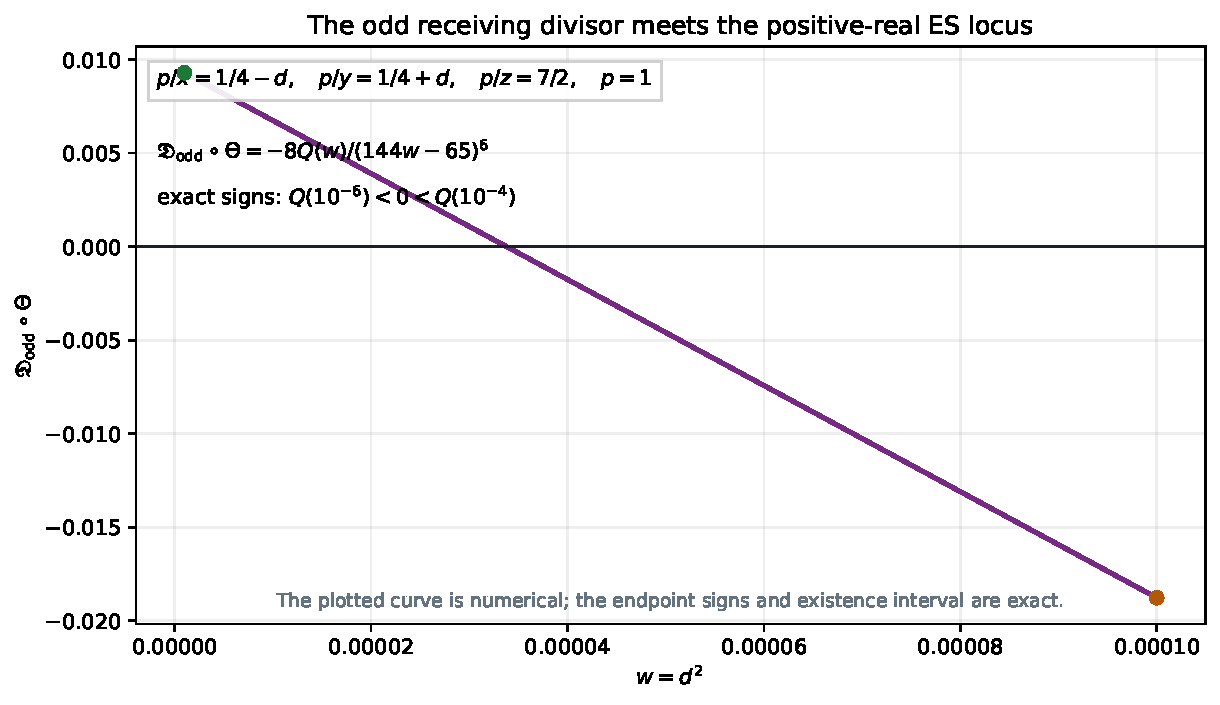
\includegraphics[width=.93\textwidth]{figures/odd-receiver-positive-real-crossing.pdf}
\caption{The exact one-parameter section EZ47 of the positive-real ES locus.
The curve is rendered numerically, while the two endpoint signs printed in
the proof are exact rational inequalities.  Their sign change proves an
intersection with the receiving divisor; it does not prove a rational or
integral intersection.  Reproduce with
\texttt{tools/generate\_20260920\_illustrations.py} and certify with
\texttt{verify\_odd\_receiver\_es\_pullback.py}.}
\label{fig:odd-receiver-positive-real-crossing}
\end{figure}
